\documentclass[border=15pt, multi, tikz]{standalone}
\usepackage{import}
\subimport{../../layers/}{init}
\usetikzlibrary{positioning}
\usetikzlibrary{3d} %for including external image 

\def\ConvColor{rgb:yellow,5;red,2.5;white,5}
\def\ConvReluColor{rgb:yellow,5;red,5;white,5}
\def\ReluColor{rgb:orange,5;red,5;white,5}
\def\FcColor{rgb:blue,5;green,2.5;white,5}
\def\PoolColor{rgb:red,1;black,0.3}
\def\DcnvColor{rgb:blue,5;green,2.5;white,5}
\def\SoftmaxColor{rgb:magenta,5;black,7}
\def\SumColor{rgb:blue,5;green,15}

\begin{document}
\begin{tikzpicture}
\tikzstyle{connection}=[ultra thick,every node/.style={sloped,allow upside down},draw=\edgecolor,opacity=0.7]
%%%%%%%%%%%%%%%%%%%%%%%%%%%%%%%%%%%%%%%%%%%%%%%%%%%%%%%%%%%%%%%%%%%%%%%%%%%%%%%%%%%%%%%%
%% Draw Layer Blocks
%%%%%%%%%%%%%%%%%%%%%%%%%%%%%%%%%%%%%%%%%%%%%%%%%%%%%%%%%%%%%%%%%%%%%%%%%%%%%%%%%%%%%%%%
\node[canvas is zy plane at x=0] (temp) at (-3,0,0) {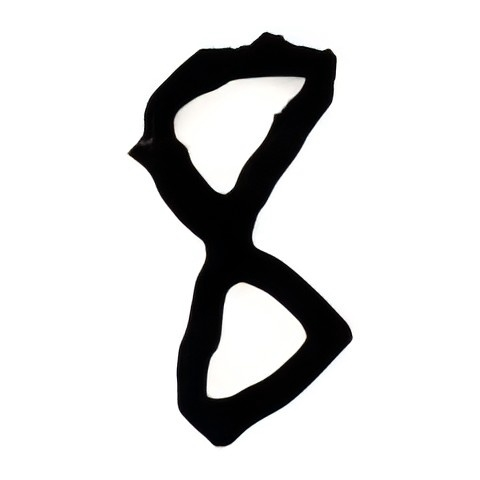
\includegraphics[width=8cm,height=8cm]{8.jpg} };

% Input Layer
\pic[shift={(0,0,0)}] at (0,0,0) {RightBandedBox={
    name=input,
    caption=Input,
    xlabel={1},
    ylabel=32,
    zlabel=32,
    fill=\ConvColor,
    bandfill=\ReluColor,
    height=32,
    width=1,
    depth=32
    }
};

% First convolution layer (6 feature maps)
\pic[shift={(1,0,0)}] at (input-east) {RightBandedBox={
    name=conv1,
    caption=Conv1 (6),
    xlabel={6},
    ylabel=28,
    zlabel=28,
    fill=\ConvColor,
    bandfill=\ReluColor,
    height=28,
    width=6,
    depth=28
    }
};

% First pooling layer
\pic[shift={(1.5,0,0)}] at (conv1-east) {RightBandedBox={
    name=pool1,
    caption=Pool1,
    xlabel={6},
    ylabel=14,
    zlabel=14,
    fill=\PoolColor,
    bandfill=\PoolColor,
    height=14,
    width=6,
    depth=14
    }
};

% Second convolution layer (16 feature maps)
\pic[shift={(2,0,0)}] at (pool1-east) {RightBandedBox={
    name=conv2,
    caption=Conv2 (16),
    xlabel={16},
    ylabel=10,
    zlabel=10,
    fill=\ConvColor,
    bandfill=\ReluColor,
    height=10,
    width=16,
    depth=10
    }
};

% Second pooling layer
\pic[shift={(2.5,0,0)}] at (conv2-east) {RightBandedBox={
    name=pool2,
    caption=Pool2,
    xlabel={16},
    ylabel=5,
    zlabel=5,
    fill=\PoolColor,
    bandfill=\PoolColor,
    height=5,
    width=16,
    depth=5
    }
};

% Flatten layer
\pic[shift={(3,0,-1)}] at (pool2-east) {RightBandedBox={
    name=flatten,
    caption=Flatten,
    xlabel={1},
    ylabel=1,
    zlabel=400,
    fill=\ConvColor,
    bandfill=\ReluColor,
    height=1,
    width=1,
    depth=40
    }
};

% First fully connected layer (400->120 neurons)
\pic[shift={(3.5,0,0)}] at (flatten-east) {RightBandedBox={
    name=fc3,
    caption=FC3 (400×120),
    xlabel={1},
    ylabel=1,
    zlabel=120,
    fill=\FcColor,
    bandfill=\ReluColor,
    height=1,
    width=1,
    depth=12
    }
};

% Second fully connected layer (120->84 neurons)
\pic[shift={(4,0,0)}] at (fc3-east) {RightBandedBox={
    name=fc4,
    caption=FC4 (120×84),
    xlabel={84},
    ylabel=1,
    zlabel=1,
    fill=\FcColor,
    bandfill=\ReluColor,
    height=1,
    width=1,
    depth=8.4
    }
};

% Output layer with softmax
\pic[shift={(5,0,0)}] at (fc4-east) {RightBandedBox={
    name=output,
    caption=Softmax,
    xlabel={1},
    ylabel=1,
    zlabel=10,
    fill=\SoftmaxColor,
    bandfill=\SoftmaxColor,
    height=1,
    width=1,
    depth=8.4
    }
};

%%%%%%%%%%%%%%%%%%%%%%%%%%%%%%%%%%%%%%%%%%%%%%%%%%%%%%%%%%%%%%%%%%%%%%%%%%%%%%%%%%%%%%%%
%% Draw connections
%%%%%%%%%%%%%%%%%%%%%%%%%%%%%%%%%%%%%%%%%%%%%%%%%%%%%%%%%%%%%%%%%%%%%%%%%%%%%%%%%%%%%%%%
\draw [connection]  (input-east)    -- node {\midarrow} (conv1-west);
\draw [connection]  (conv1-east)    -- node {\midarrow} (pool1-west);
\draw [connection]  (pool1-east)    -- node {\midarrow} (conv2-west);
\draw [connection]  (conv2-east)    -- node {\midarrow} (pool2-west);
\draw [connection]  (pool2-east)    -- node {\midarrow} (flatten-west);
\draw [connection]  (flatten-east)  -- node {\midarrow} (fc3-west);
\draw [connection]  (fc3-east)      -- node {\midarrow} (fc4-west);
\draw [connection]  (fc4-east)      -- node {\midarrow} (output-west);
%%%%%%%%%%%%%%%%%%%%%%%%%%%%%%%%%%%%%%%%%%%%%%%%%%%%%%%%%%%%%%%%%%%%%%%%%%%%%%%%%%%%%%%%

\end{tikzpicture}
\end{document}
